% Chapter 2
\chapter{Background} % Main chapter title
\label{Chapter2} % For referencing the chapter elsewhere, use \ref{Chapter1} 
\lhead{Chapter 2. \emph{State of Art}} % This is for the header on each page - perhaps a shortened title

\par 

%----------------------------------------------------------------------------------------
\section{Business justification for your work}
%----------------------------------------------------------------------------------------

\par 

\par 

%----------------------------------------------------------------------------------------
\subsection{Market research}
%----------------------------------------------------------------------------------------

\par 

\par 

%----------------------------------------------------------------------------------------
\section{Research methods}
%----------------------------------------------------------------------------------------


\par There are different methodologies, which can be used in order to conduct a research. Most of the researches apply scientific method see Figure \ref{fig:sci-method.png} .


\begin{figure}[H]
    \centering
    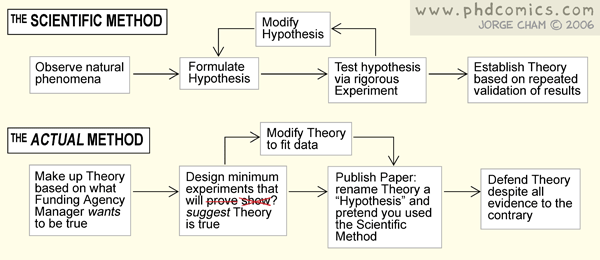
\includegraphics[scale=0.9]{Figures/sci-method.png}
    %\rule{35em}{0.5pt}
    \caption[Sci method]{Sci method}
    \label{fig:sci-method.png}
\end{figure}

\par Depending on the study, there are different techniques, which can be applied. In our case, during our project we did conduct few studies. In order to conduct our research we preside following steps: 

\begin{enumerate}
    \item Formulating the research problem;
    \item Extensive literature survey;
    \item Developing hypothesis;
    \item Preparing the research design;
    \item Determining sample design;
    \item Collecting data;
    \item Execution of the project and Implementation of the project;
    \item Analysis of data;
    \item Hypothesis testing;
    \item Generalization and interpretation;
    \item Preparation of the report / presentation of our results \cite{Research-Methodology-Methods-and-Techniques}.
\end{enumerate}

\par To be more precise, we had two major different studies in our hands. First one was about user experience of our application. Second one was about drawing conclusions and results from insulin sensor data. 

\par We used qualitative and quantitative research method approaches to our problems due to data type. So, we are going to explain research types and their differences (see Table \ref{table:2.1}) As well as, how we applied this methods.

\begin{table}[H]
\begin{tabular}{|l|l|}
\hline
\textbf{Qualitative} & \textbf{Quantitative} \\ \hline
\begin{tabular}[c]{@{}l@{}}Direct observation, Open-ended surveys, \\ Focus group, In-depth interviews,\\ Oral history, Participant observation, \\ Ethnographic observation, Content analysis.\\ In UX we could apply: Interviews \\ (directed, non-directed, ethnographic), \\ Surveys, Questionnaires, Usability Tests \\ (moderated, unmoderated, guerrilla), Card \\ sorting, Tree testing, A/B testing, \\ \\ \href{ https://www.oreilly.com/library/view/ux-research/9781491951286/ch04.html}{Persona development}, and \href{https://www.nngroup.com/articles/which-ux-research-methods/}{so on} ... \end{tabular} & \begin{tabular}[c]{@{}l@{}}Surveys, structured interviews, \\ observations, reviews of records / \\ numeric information:\\ Study population, Sampling, \\ Data collection, Data analysis,\\ \\  \href{https://libguides.usc.edu/writingguide/quantitative}{Statistical analysis}\end{tabular} \\ \hline
\begin{tabular}[c]{@{}l@{}}Primarily inductive process used to \\ formulate theory / hypotheses\end{tabular} & \begin{tabular}[c]{@{}l@{}}Primarily deductive process used to test \\ pre-specified concepts, constructs, and \\ hypotheses that make up a theory\end{tabular} \\ \hline
\begin{tabular}[c]{@{}l@{}}More subjective: describes a problem / \\ condition from the point of view of \\ those experiencing it\end{tabular} & \begin{tabular}[c]{@{}l@{}}More objective: provides observed \\ effects (interpreted by researchers) \\ of a program on a problem or condition\end{tabular} \\ \hline
Text-based, Descriptive data & Number-based, Numerical data \\ \hline
More in-depth information on a few cases & \begin{tabular}[c]{@{}l@{}}Less in-depth but more breadth of \\ information across a large number\\  of cases\end{tabular} \\ \hline
\begin{tabular}[c]{@{}l@{}}Unstructured or semi-structured \\ response options\end{tabular} & Fixed response options \\ \hline
No statistical tests & Statistical tests are used for analysis \\ \hline
\begin{tabular}[c]{@{}l@{}}Can be valid and reliable: \\ largely depends on skill \\ and rigor of the researcher\end{tabular} & \begin{tabular}[c]{@{}l@{}}Can be valid and reliable: \\ largely depends on the measurement \\ device or instrument used\end{tabular} \\ \hline
\begin{tabular}[c]{@{}l@{}}Time expenditure lighter on the \\ planning end and heavier \\ during the analysis phase\end{tabular} & \begin{tabular}[c]{@{}l@{}}Time expenditure heavier on the \\ planning phase and lighter on the \\ analysis phase\end{tabular} \\ \hline
Less generalizable & More generalizable \\ \hline
\end{tabular}
\caption{ \href{https://www.orau.gov/cdcynergy/soc2web/content/phase05/phase05_step03_deeper_qualitative_and_quantitative.htm}{Difference between quantitative and qualitative research methods applied}}
\label{table:2.1}
\end{table}

% https://www.publichealthnotes.com/differences-qualitative-quantitative-research/

%----------------------------------------------------------------------------------------
\subsection{Qualitative research - User Experience}
%----------------------------------------------------------------------------------------

\par We formulated a research problem as - smoothing user experience of glucose monitoring systems in Android devises.  While doing literature survey, we stumbled upon a study with a schematic diagram of the tailored mobile coaching system on diabetes management (see Figure \ref{fig:Schematic-diagram-of-the-tailored-mobile-coaching-system.jpg}). Their application design was developed for teaching about diabetes, however we realized - that we could tailor their solution a little and get an application for our case. As a result, we decided to formulate hypothesis, where we deduced, that an a diabetic Android application for controlling glucose level should combine functionality of: statistics on Iot devise, everyday dosages of insulin, diary on food and exercises, medical record keeper, notifications for regular and emergency situations. 

\par For a research design we used different methods. First, we conducted direct Interviews. Second, we used persona development method in order to identify categories of our main uses. Finally, we conducted usability tests for different prototypes. In each step, we changed the design by analyzing responses of our focus group. Furthermore , we challenged our hypothesis one more time. Next, we generalized and interpreted results, by which our first hypothesis were true. Therefor, we implemented final version of out design. 


\par Qualitative research method was helpful in our case because we were dealing with text-base data. As well as, we have to take into account, that it is more subjective data. Also, we (researchers) had to interpreted the data, which been collected from individuals with diabetes and their reaction to InsuPad with Android Application. Moreover, we were shoving images of different prototypes as well as different design of InsuPad itself. The final result of design of application is presented in next chapters.

%----------------------------------------------------------------------------------------
\section{Software Development Methodology}
%----------------------------------------------------------------------------------------

\par During development process we have to use a methodology in order to satisfy an end quality of the product. In our case, due to a limited time and specific requirements, which have to be implemented, we preseed with Dr. Winston W. Royce first described the Waterfall Model (see Figure \ref{fig:Unmodified-Waterfall-Development-Model.jpg}). This model with no iteration, sometimes called “stagewise”. However, in Dr. Winston W. Royce’s paper did not use the term “waterfall”, he described the process itself. It was firs mentioned in relation to developing software in “Managing the Development of Large Software Systems”. The model includes the following steps: System requirements, Software Requirements, Analysis, Program Design, Coding, Testing, and Operations. As we can see, an unmodified waterfall process does not allow iteration like: going back to previous steps. This places a heavy planning burden on the earlier steps, as well as risks management. Also, since each subsequent step cannot begin until the previous step ends, any delays in earlier steps cause delays to the later steps.

\begin{figure}[H]
    \centering
    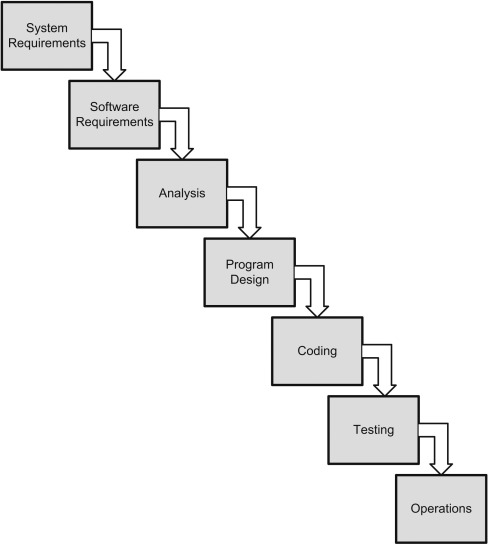
\includegraphics[scale=0.9]{Figures/Unmodified-Waterfall-Development-Model.jpg}
    %\rule{35em}{0.5pt}
    \caption[Unmodified-Waterfall-Development-Model]{Unmodified waterfall development model by Dr. Winston W. Royce. \cite{Unmodified-Waterfall-Development-Model}}
    \label{fig:Unmodified-Waterfall-Development-Model.jpg}
\end{figure}
% https://www.sciencedirect.com/topics/computer-science/waterfall-model

\par At the same time, we have the true demonstration of final thesis draft time-line in a Figure \ref{fig:thesis-word-count.png}. Of course  \href{https://www.lesswrong.com/posts/CPm5LTwHrvBJCa9h5/planning-fallacy}{planning fallacy} can be applied here.
% https://www.lesswrong.com/posts/CPm5LTwHrvBJCa9h5/planning-fallacy

\begin{figure}[H]
    \centering
    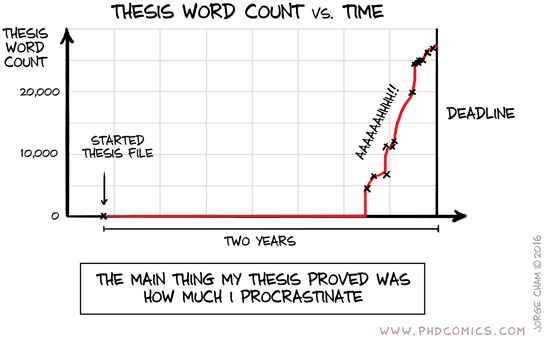
\includegraphics[scale=0.9]{Figures/thesis-word-count.png}
    %\rule{35em}{0.5pt}
    \caption[thesis-word-count]{\href{http://phdcomics.com/comics/archive_print.php?comicid=1915}{Thesis time-line}}
    \label{fig:thesis-word-count.png}
\end{figure}

%----------------------------------------------------------------------------------------
\section{Literature review}
%----------------------------------------------------------------------------------------
\pad In this section, we are going to look into researches of similar cases and similar applications. As well as, we are going to look into technologies and researches, which were used to make this product. 


%----------------------------------------------------------------------------------------
\subsection{}
%----------------------------------------------------------------------------------------


\par 

\par 

\par 

\par 

%C\item Chapter 1: Introduction, Background, Motivation, Problem statement, Goals, Restrictions, Overview;
%C\item Chapter 2: Literature Survey and Background:  Research method, Methodology of Software Development, Literature review, Related Works
%C\item Chapter 3: Theoretical Foundations: Background Material, State of art, Internet of Things, Theory on hardware, Serverless architecture
%C\item Chapter 4: Protocol and systems(services and programs) used to build the system.
%C\item Chapter 5: Formal Model: Theoretical Development, Implementation / Use cases, Testing
%C\item Chapter 6: Algorithmic Considerations
%C\item Chapter 7: Implementation Issues, Results and Evaluation
%C\item Chapter 8: Discussion, Critical Appraisal, Conclusions
%C\item Chapter 9: Future Work 

%Chapter 1. Introduction & Overview
%Chapter 2. Literature Survey
%Chapter 3. Theoretical Foundations: Background Material
%Chapter 4. Formal Model: Theoretical Development (use additional chapters if necessary)
%Chapter 5. Algorithmic Considerations
%Chapter 6. Implementation Issues
%Chapter 7. Evaluation
%Chapter 8. Discussion & Critical Appraisal
%References
%Appendices
% Key Software listings
% Mechanical schematics
% Mathematical proofs